\section{}
\textit{Consider steady, two-dimensional, incompressible flow due to a spiraling line vortex/sink flow centered on the $z$-axis. Streamlines and velocity components are shown in the following figure. The velocity field is $u_r = C/r$ and $u_{\theta} = K/r$, where $C$ and $K$ are constants. Calculate the pressure as a function of $r$.}

\begin{figure}[h]
    \centering
    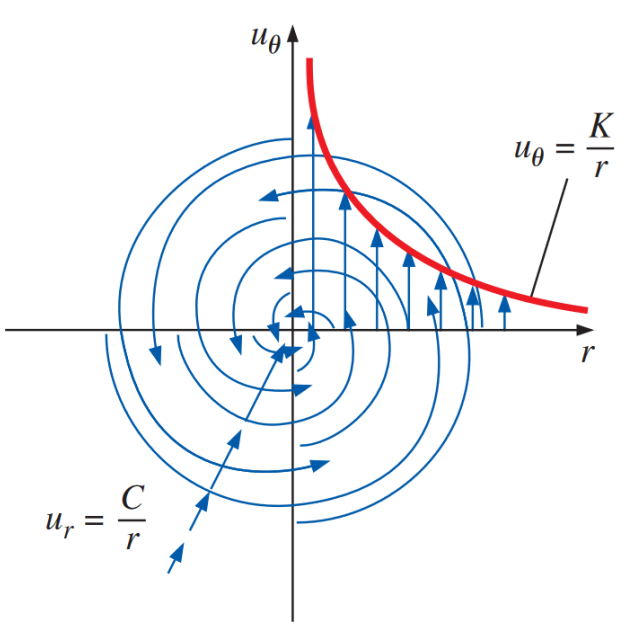
\includegraphics[width=0.5\textwidth]{Questions/Figures/Q1 Problem Diagram.png}
\end{figure}

\subsection*{Solution}
First we list our assumptions and their consequences:
\begin{table}[h]
    \centering
    \begin{tabular}{ccc}
        \toprule
        Number & Assumption & Consequence \\
        \hline
        \#1 & Steady flow & $\frac{\partial}{\partial t} = 0$ \\
        \#2 & Incompressible flow & $\rho = \text{constant}$ \\
        \#3 & Two-dimensional flow & $u_z = 0$, $\partial_z \vec{v} = 0$ \\
        \#4 & No Gravity on $r$, $\theta$ & $g_r = g_{\theta} = 0$ \\
        \#5 & $u_r$ has $\theta$ Independence & $\frac{\partial u_r}{\partial \theta} = 0$ \\
        \#6 & $u_{\theta}$ has $\theta$ Independence & $\frac{\partial u_{\theta}}{\partial \theta} = 0$ \\
        \bottomrule
    \end{tabular}
\end{table}
Starting with the continuity equation, we have
\begin{align*}
    % \frac{1}{r} \frac{\partial (r u_r)}{\partial r} + \frac{1}{r} \frac{\partial u_{\theta}}{\partial \theta} + \frac{\partial u_z}{\partial z} = 0
    \frac{1}{r} \frac{\partial (r u_r)}{\partial r} + \frac{1}{r} \cancelto{\text{\#6}}{\frac{\partial u_{\theta}}{\partial \theta}} + \cancelto{\text{\#3}}{\frac{\partial u_z}{\partial z}} = 0
\end{align*}
Now the momentum equation in the $r$ direction is
% $r$ & \(\displaystyle\begin{aligned} \frac{\partial u_r}{\partial t} + u_r \frac{\partial u_r}{\partial r} + \frac{u_{\theta}}{r} \frac{\partial u_r}{\partial \theta} - \frac{u_{\theta}^2}{r} + u_z \frac{\partial u_r}{\partial z} &= -\frac{1}{\rho} \frac{\partial P}{\partial r} + g_r \\ &\quad + \frac{\mu}{\rho} \left[\frac{1}{r} \frac{\partial}{\partial r}\left(r \frac{\partial u_r}{\partial r}\right) - \frac{u_r}{r^2} + \frac{1}{r^2} \frac{\partial^2 u_r}{\partial \theta^2} - \frac{2}{r^2} \frac{\partial u_{\theta}}{\partial \theta} + \frac{\partial^2 u_r}{\partial z^2}\right]  \end{aligned}\) \\[7ex]
\begin{align*}
    \cancelto{\text{\#1}}{\frac{\partial u_r}{\partial t}} + u_r \frac{\partial u_r}{\partial r} + \frac{u_{\theta}}{r} \cancelto{\text{\#5}}{\frac{\partial u_r}{\partial \theta}} - \frac{u_{\theta}^2}{r} + u_z \cancelto{\text{\#3}}{\frac{\partial u_r}{\partial z}} &= -\frac{1}{\rho} \frac{\partial P}{\partial r} + \cancelto{\text{\#4}}{g_r} \\
    &\quad + \frac{\mu}{\rho} \left[\frac{\partial}{\partial r}\cancelto{\text{Cont.}}{\left(\frac{1}{r}\frac{\partial}{\partial r}(r u_r)\right)} + \frac{1}{r^2} \cancelto{\text{\#6}}{\frac{\partial^2 u_r}{\partial \theta^2}} - \frac{2}{r^2} \cancelto{\text{\#6}}{\frac{\partial u_{\theta}}{\partial \theta}} + \cancelto{\text{\#3}}{\frac{\partial^2 u_r}{\partial z^2}}\right]
\end{align*}
which simplifies to
\begin{align*}
    u_r \frac{\partial u_r}{\partial r} - \frac{u_{\theta}^2}{r} &= -\frac{1}{\rho} \frac{\partial P}{\partial r}
\end{align*}
substituting in $u_r = C/r$ and $u_{\theta} = K/r$ gives
\begin{align*}
    \frac{C}{r} \left(\frac{-C}{r^2}\right) - \frac{K^2}{r^3} &= -\frac{1}{\rho} \frac{\partial P}{\partial r} \\
    \rho \frac{C^2 + K^2}{r^3} &= \frac{\partial P}{\partial r} 
\end{align*}
Solving,
\begin{align*}
    \Aboxed{P &= -\frac{\rho}{2} \left(\frac{C^2 + K^2}{r^2}\right) + C_1}
\end{align*}
From the Navier-Stokes equation in the $\theta$ direction, it can be shown that P is only a function of $r$ and not $\theta$. Thus, $C_1$ is some constant and not a function of $\theta$.